\begin{figure}[H]
    \centering
    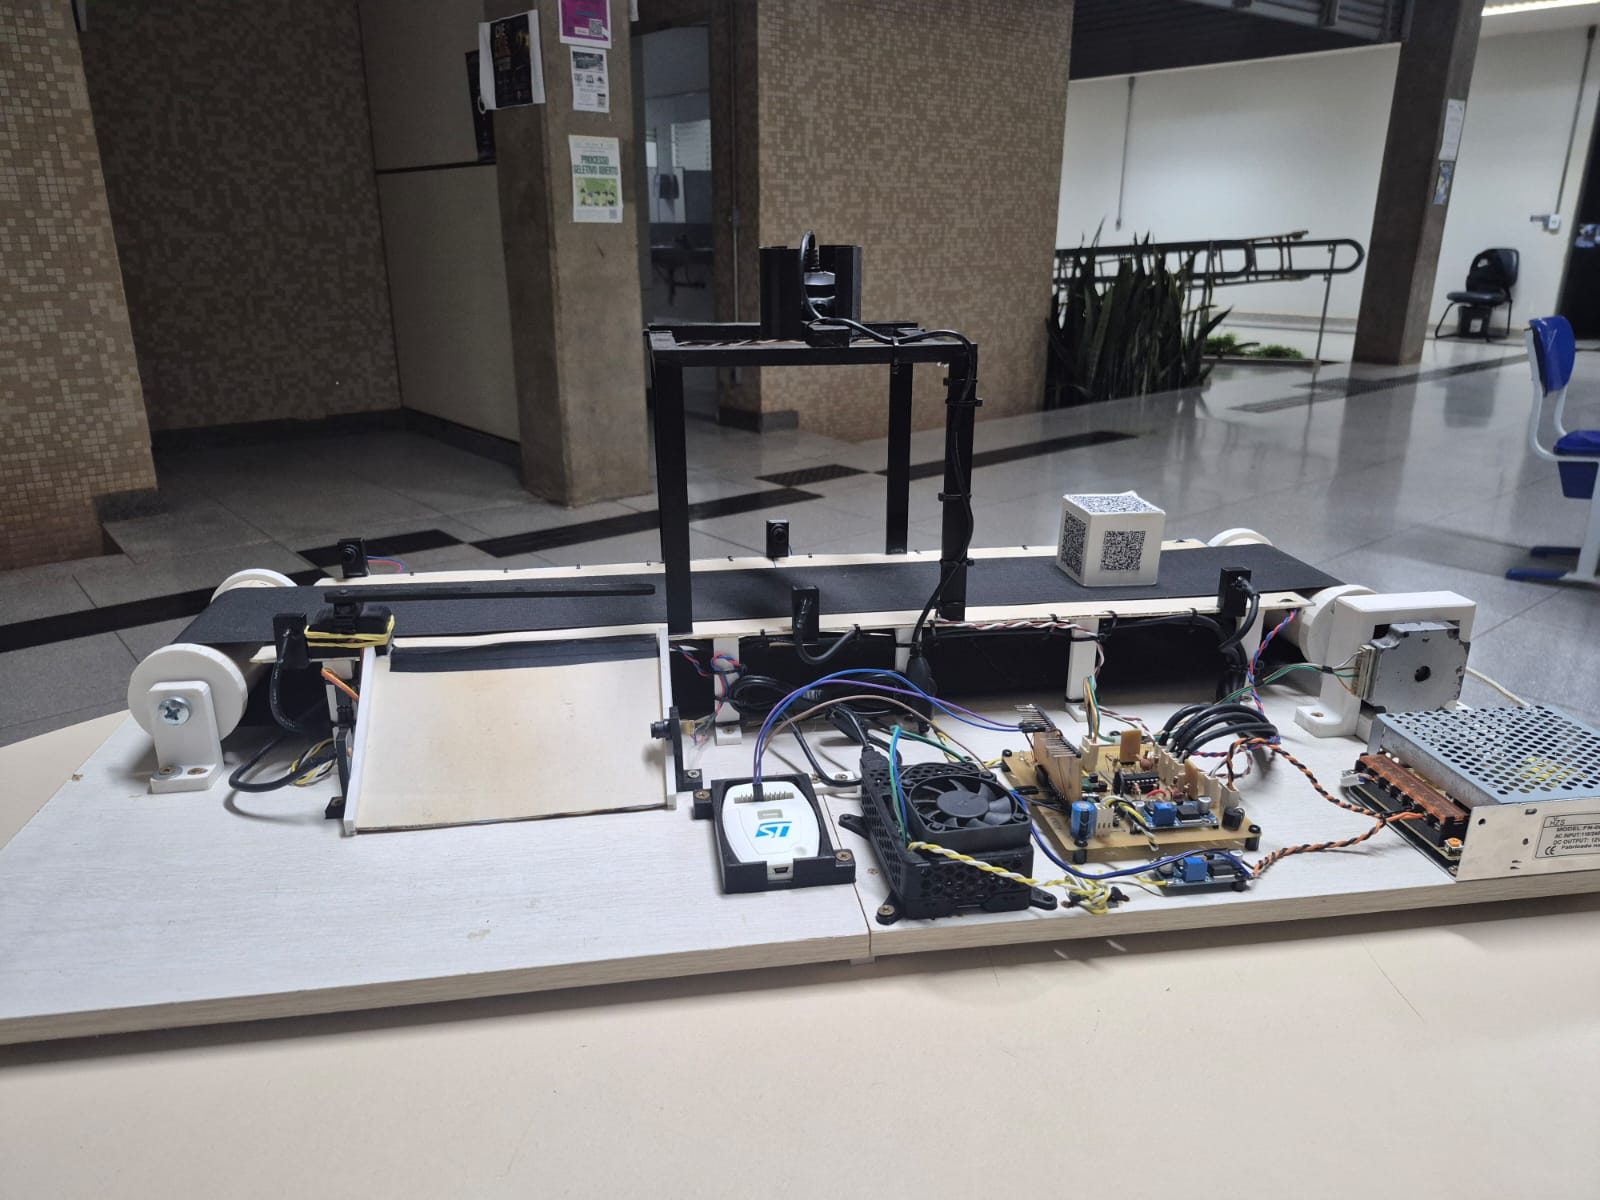
\includegraphics[width=1\linewidth]{figuras/esteira.jpeg}
    \caption{Foto da esteira}
    \label{fig:esteira}
\end{figure}\subsection{Descrição de \textit{hardware}}\label{subsec:hardware}

O sistema é composto por uma arquitetura híbrida que divide as responsabilidades entre um microprocessador Broadcom BCM2837, hospedado na placa Raspberry Pi 3B e responsável pelas tarefas de alto nível, e um microcontrolador STM32G070, dedicado ao controle em tempo real dos dispositivos físicos da esteira. O diagrama de blocos da Fig.~\ref{fig:Diag_blocks} ilustra de forma simplificada a arquitetura do sistema.

\begin{figure}[H]
    \centering
    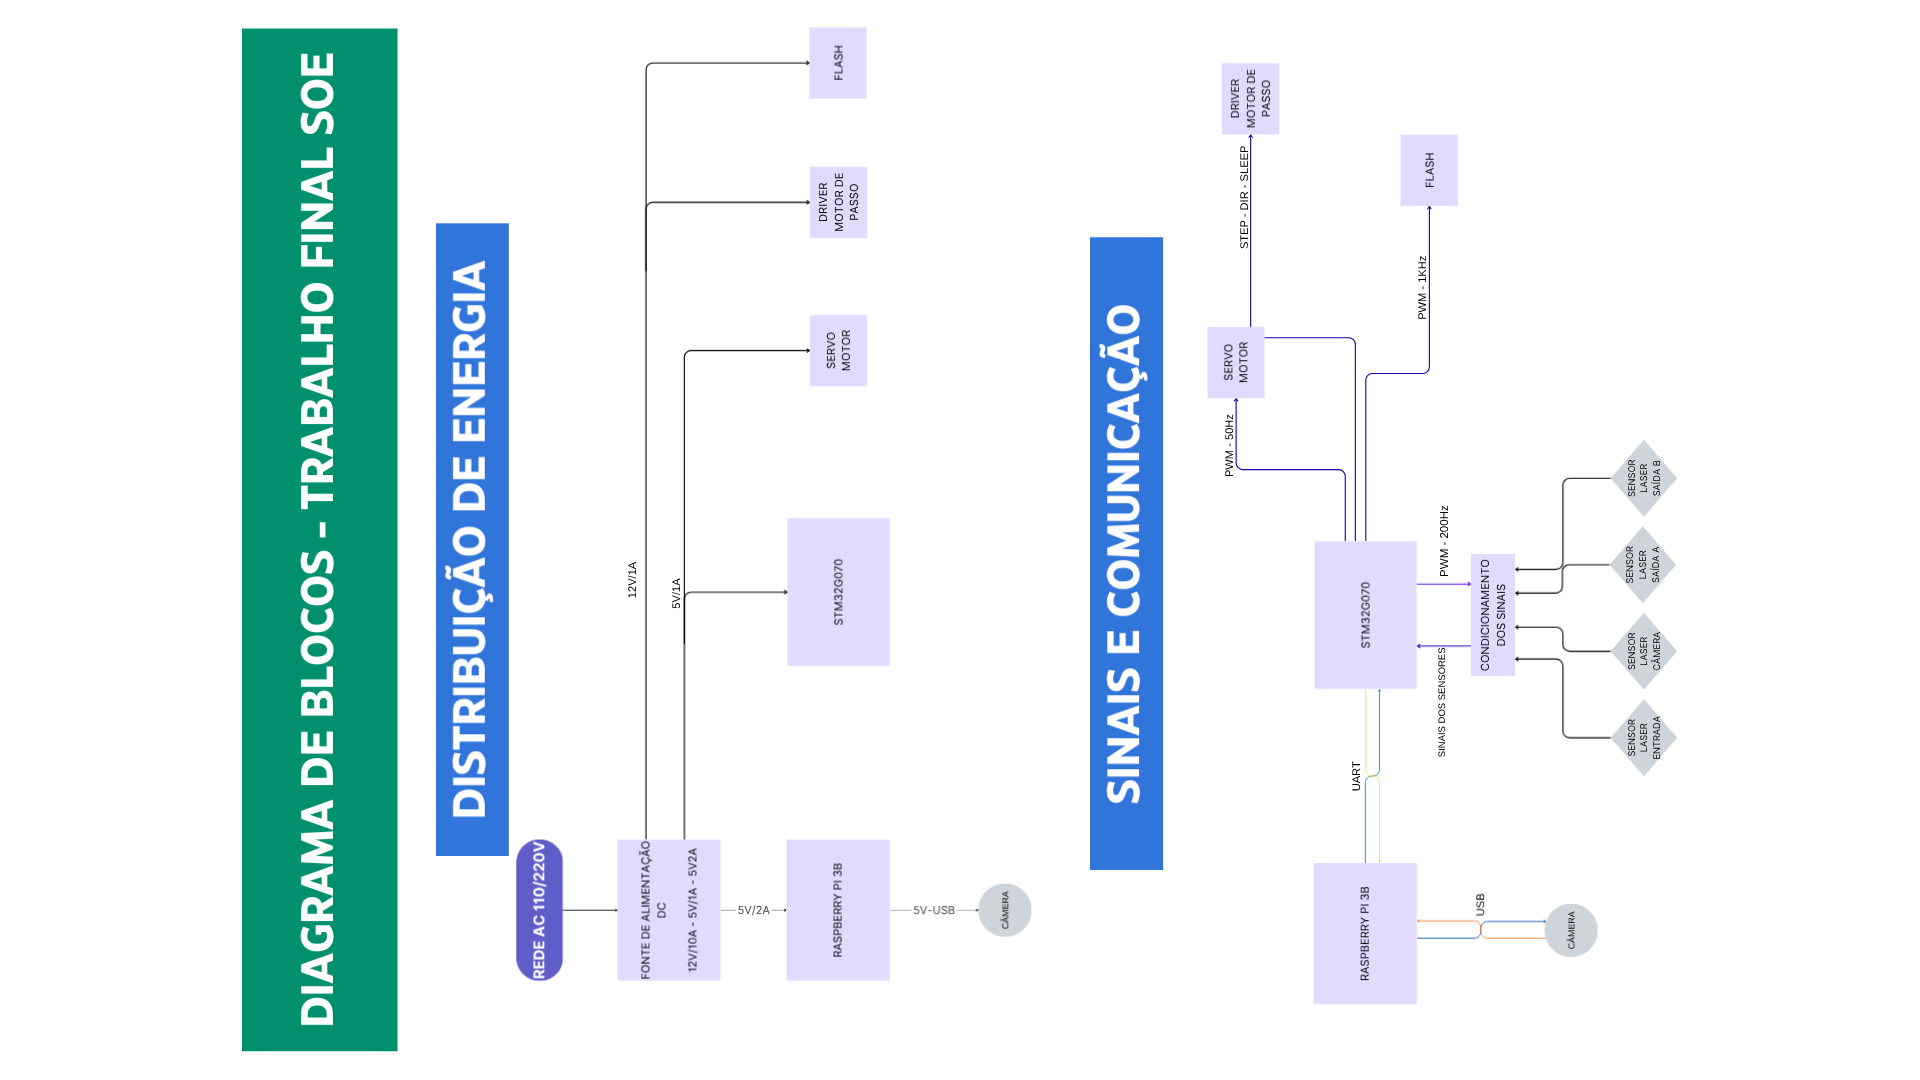
\includegraphics[angle=-90, width=1\linewidth]{figuras/DIAGRAMA DE BLOCOS.png}
    \caption{Diagrama de blocos do \textit{hardware}.}
    \label{fig:Diag_blocks}
\end{figure}

\newpage
A placa Raspberry Pi 3B foi escolhida devido à ampla documentação disponível, à acessibilidade ao \textit{hardware}, uma vez que um dos integrantes da dupla já dispunha de uma unidade em funcionamento, e ao suporte nativo ao sistema operacional Linux, requisito para a execução da interface gráfica e dos algoritmos de visão computacional desenvolvidos neste projeto.

A câmera utilizada para a leitura e processamento de imagem é uma \textit{webcam} genérica da marca Multilaser, com interface USB. A escolha foi motivada pela ausência de necessidade de \textit{drivers} proprietários para o correto funcionamento com o Linux embarcado e pela disponibilidade imediata para o projeto.

O microcontrolador STM32G070 foi escolhido por sua variedade de periféricos adequados à aplicação, como comunicação UART, \textit{timers} de uso geral e recurso de DMA (\textit{Direct Memory Access}), que permite processar informações obtidas pelos periféricos sem ocupar a CPU. Além dessas características, o STM32G070 opera a uma frequência de CPU de 64\,MHz e é suportado pelo ambiente de desenvolvimento integrado STM32CubeIDE, da STMicroelectronics, referência mundial na fabricação e suporte de microcontroladores para a indústria. O esquemático de conexão do microcontrolador pode ser observado na Fig.~\ref{fig:sch_stm32}. Os \textit{timers} são utilizados da seguinte forma:

\begin{itemize}
    \item \textbf{TIM15:} gera o sinal PWM de frequência fixa (200\,Hz, \textit{duty cycle} de 50\,\%) utilizado para modular os lasers dos sensores;
    \item \textbf{TIM3:} configurado em modo \textit{Input Capture} com DMA, realiza a medição de frequência dos quatro sensores laser simultaneamente;
    \item \textbf{TIM16:} gera o sinal PWM de 50\,Hz com \textit{duty cycle} variável para o controle do servo motor;
    \item \textbf{TIM17:} gera o sinal PWM de 1K\,Hz com \textit{duty cycle} variável para o controle da luminária;
    \item \textbf{TIM6:} opera a 1\,MHz e dispara interrupções periódicas para o controle preciso dos pulsos enviados ao \textit{driver} do motor de passo.
\end{itemize}

\begin{figure}[H]
    \centering
    
\includegraphics[width=0.75\linewidth]{figuras/Esquematico_microcontrolador.png}
    \caption{Esquemático do microcontrolador STM32G070.}
    \label{fig:sch_stm32}
\end{figure}

A interface de programação e depuração do STM32G070 é realizada via \textit{Serial Wire Debug} (SWD), conectada ao ST-Link V2 conforme o esquemático da Fig.~\ref{fig:sch_swd}. Os sinais SWCLK, SWDIO e NRST permitem gravar o \textit{firmware} e depurar o sistema em tempo real diretamente pelo STM32CubeIDE.

\begin{figure}[H]
    \centering
    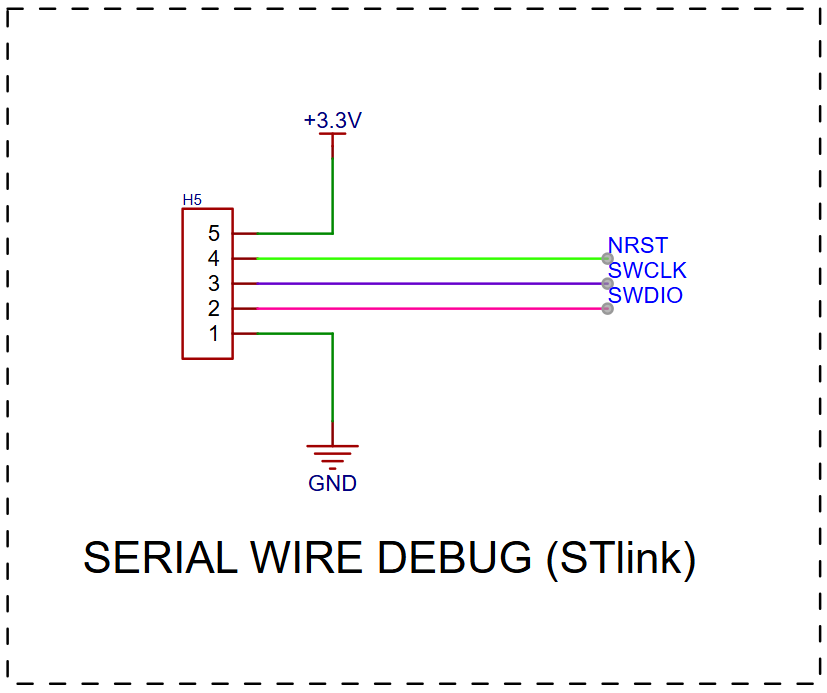
\includegraphics[width=0.75\linewidth]{figuras/serial_wire_debug.png}
    \caption{Esquemático da interface \textit{Serial Wire Debug} (ST-Link).}
    \label{fig:sch_swd}
\end{figure}

A comunicação serial entre o STM32G070 e o Raspberry Pi 3B é realizada via UART, convertida para USB por meio de um módulo conversor dedicado, cujo esquemático é apresentado na Fig.~\ref{fig:sch_uart_usb}. Esse conversor permite que o Raspberry Pi acesse a porta serial do microcontrolador como um dispositivo \texttt{/dev/ttyUSB}, sem necessidade de adaptação de nível lógico adicional, uma vez que tanto o STM32 quanto o conversor operam em 3,3\,V.

\begin{figure}[H]
    \centering
    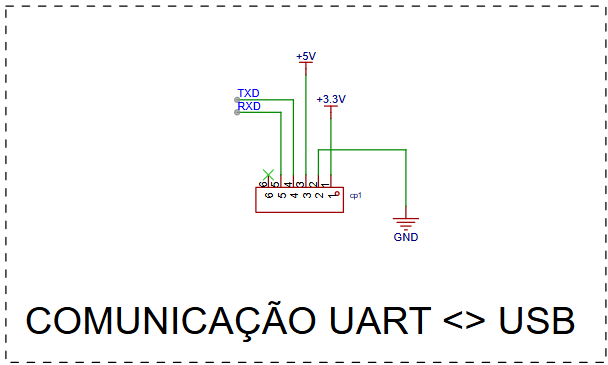
\includegraphics[width=0.65\linewidth]{figuras/comunicacao_uart.png}
    \caption{Esquemático do conversor UART $\leftrightarrow$ USB.}
    \label{fig:sch_uart_usb}
\end{figure}

A alimentação do sistema é gerenciada por dois estágios de regulação, conforme o esquemático da Fig.~\ref{fig:sch_alimentacao}. A tensão de entrada de 12\,V, proveniente de uma fonte externa, é convertida para 5\,V pelo módulo \textit{buck} LM2596S, protegido por um diodo 6A10 contra inversão de polaridade. O regulador linear AMS1117-3.3 deriva os 3,3\,V necessários para a alimentação do STM32G070 e dos circuitos de sinal a partir dos 5\,V. Capacitores de desacoplamento de 100\,nF estão presentes na entrada e saída do AMS1117-3.3 para rejeição de ruído de alta frequência.

\begin{figure}[H]
    \centering
    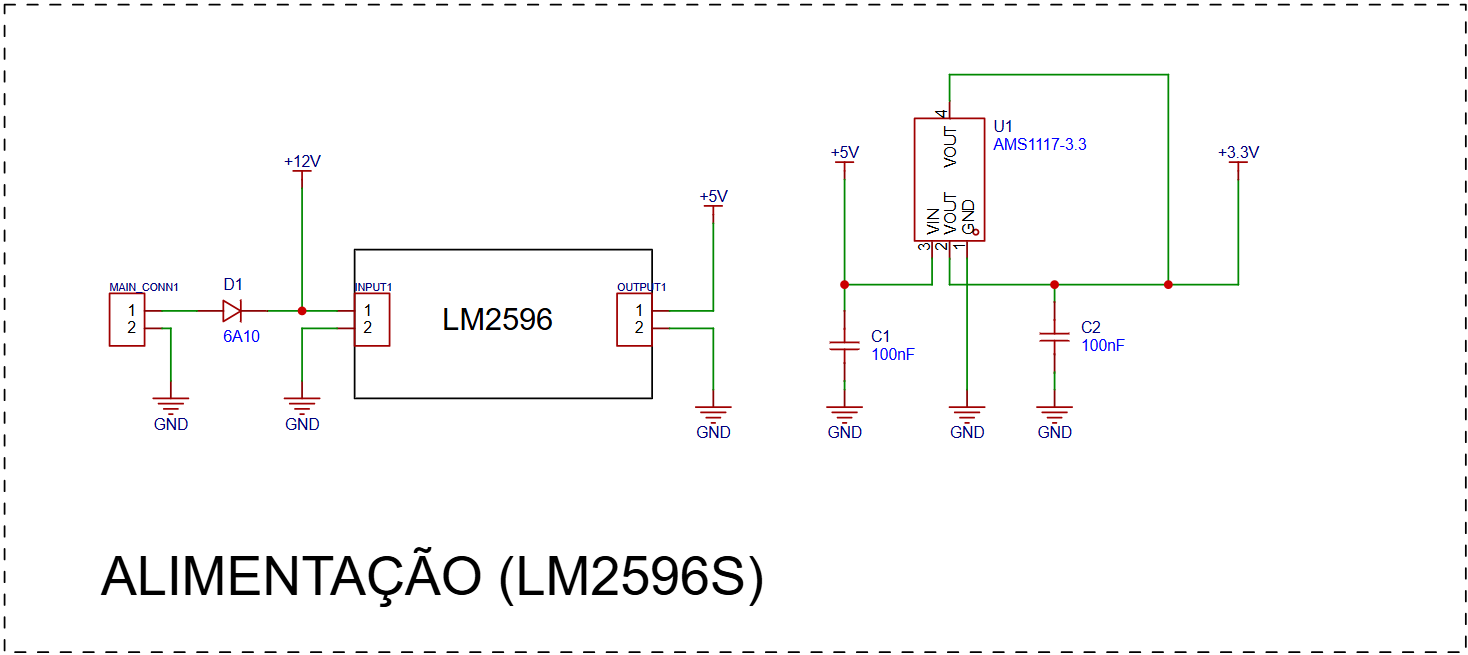
\includegraphics[width=0.85\linewidth]{figuras/alimentacao_lm2596s.png}
    \caption{Esquemático do circuito de alimentação (LM2596S + AMS1117-3.3).}
    \label{fig:sch_alimentacao}
\end{figure}

Como sistema motor do tapete da esteira, foi utilizado um motor de passo NEMA 22 controlado pelo \textit{driver} A4988, conforme o esquemático da Fig.~\ref{fig:sch_motor_passo}. Os pinos STEP, DIR e SLEEP são utilizados, respectivamente, para avançar um passo, definir a direção de rotação e habilitar ou desabilitar o \textit{driver} (liberando ou travando o eixo). Esses componentes foram escolhidos por sua disponibilidade e pela baixa complexidade operacional do \textit{driver}.

\begin{figure}[H]
    \centering
    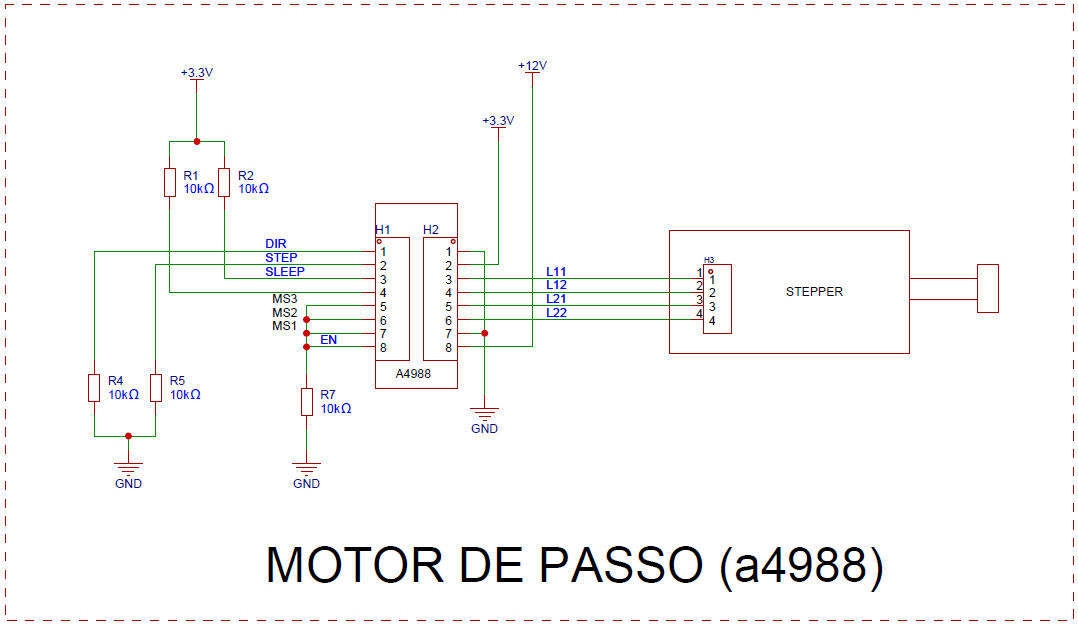
\includegraphics[width=0.85\linewidth]{figuras/Motor_de_passo_driver.png}
    \caption{Esquemático do motor de passo e do \textit{driver} A4988.}
    \label{fig:sch_motor_passo}
\end{figure}

Como atuador da cancela, foi utilizado o servo motor ES08MA (Fig.~\ref{fig:sch_servo_motor}), selecionado pela disponibilidade para o projeto e pelo torque superior ao do modelo SG90. O servo é controlado por PWM de 50\,Hz, com largura de pulso variando entre 600\,µs (0°) e 2300\,µs (180°), mapeada diretamente a partir do ângulo desejado pelo \textit{firmware}.

\begin{figure}[h]
    \centering
    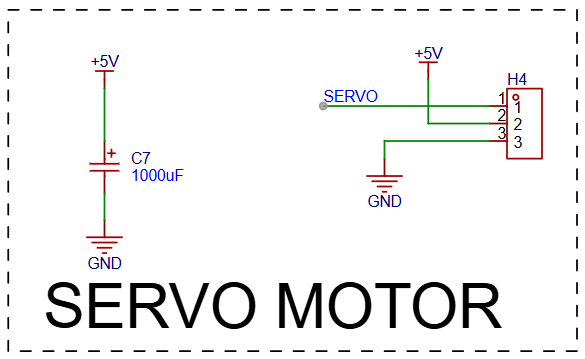
\includegraphics[width=0.4\linewidth]{figuras/servo_motor.png}
    \caption{Esquemático do servo motor ES08MA.}
    \label{fig:sch_servo_motor}
\end{figure}

Os sensores laser foram projetados para apresentar a maior simplicidade possível e para que o circuito eletrônico fosse viável de fabricação artesanal em \textit{breakout boards} com solda manual. O princípio de funcionamento é baseado em detecção síncrona por ausência de portadora: o laser modula seu feixe na frequência gerada pelo TIM15 (200\,Hz). O feixe incide sobre um LDR que, após condicionamento de sinal com amplificadores operacionais (LM324), entrega ao STM32G070 um sinal digital pulsado na faixa de 0 a 3,3\,V com frequência idêntica à portadora. Quando um objeto interrompe o feixe, a ausência do sinal pulsado, interpretada pelo \textit{firmware} como nível lógico alto permanente na entrada de captura, é identificada como presença de objeto à frente do sensor. O circuito conta com quatro instâncias desse sensor, dispostas em posições estratégicas ao longo da esteira: entrada da esteira (S1), zona de leitura do QR (S2), saída da Rota~A (S3) e saída da Rota~B (S4). O esquemático completo dos quatro sensores é apresentado na Fig.~\ref{fig:sch_sensores}.

\begin{figure}[H]
    \centering
    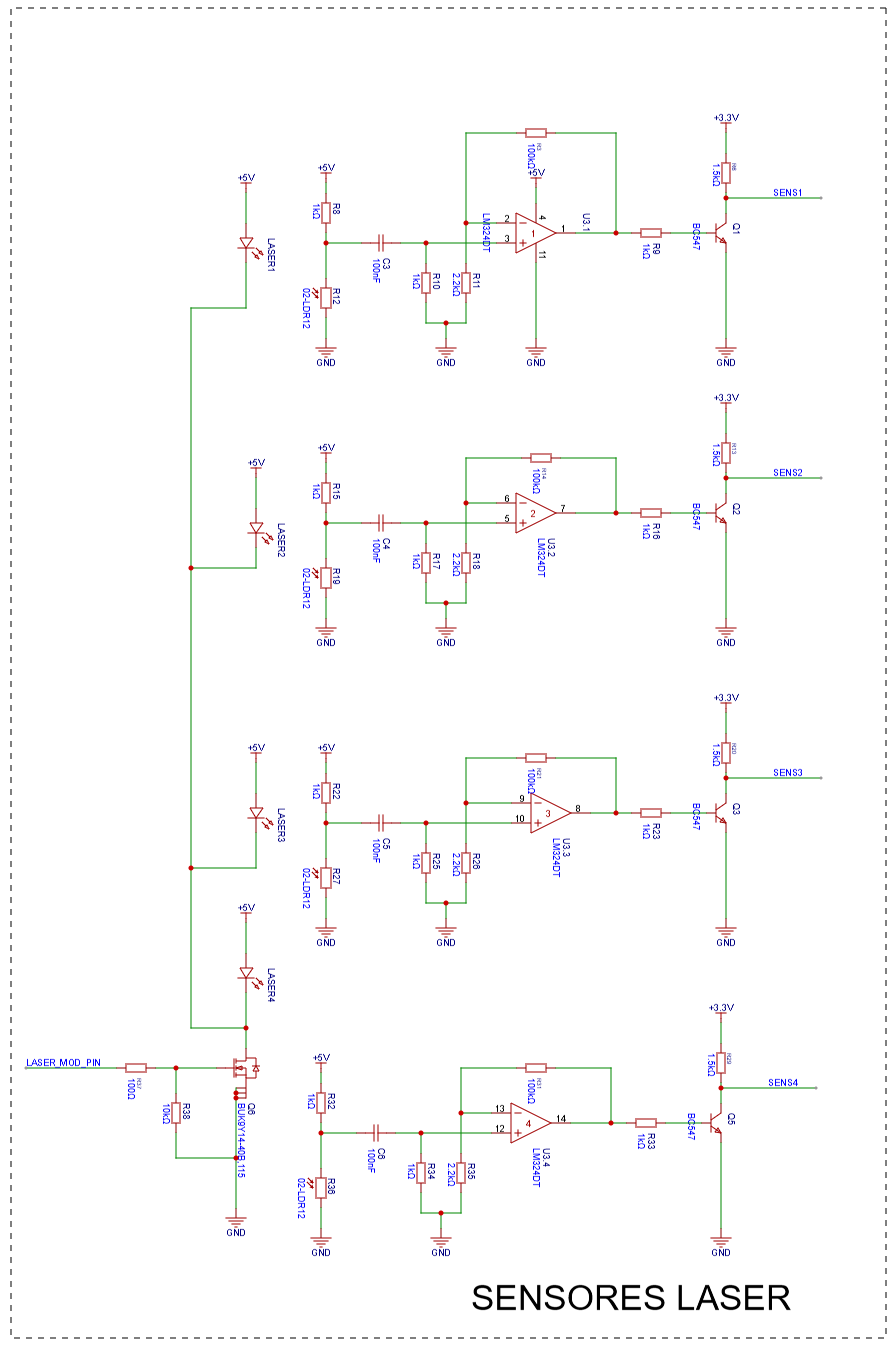
\includegraphics[width=0.9\linewidth]{figuras/sensor_laser.png}
    \caption{Esquemático dos quatro sensores laser com condicionamento de sinal (LDR + LM324).}
    \label{fig:sch_sensores}
\end{figure}

Para auxiliar a visualização do código QR pela câmera, o sistema conta com uma luminária composta por seis LEDs de uma fita LED 4000\,K. A temperatura de cor foi escolhida por apresentar maior similaridade com a luz ambiente, o que resultou em melhor qualidade de captura da câmera em comparação com fitas de 6500\,K. O acionamento da luminária é realizado por PWM controlado pelo canal 1 do TIM17 do STM32G070, por meio de um MOSFET BUK9Y14 em configuração de chave, como ilustrado no esquemático da Fig.~\ref{fig:sch_luminaria}.

\begin{figure}[H]
    \centering
    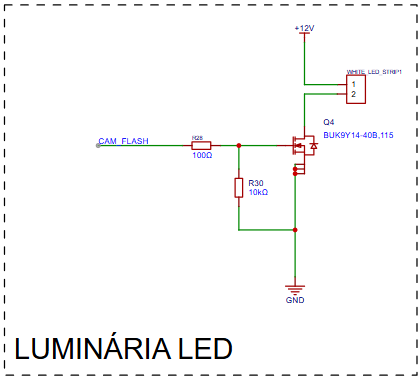
\includegraphics[width=0.55\linewidth]{figuras/luminaria_led.png}
    \caption{Esquemático do circuito de acionamento da luminária LED.}
    \label{fig:sch_luminaria}
\end{figure}

O esquemático completo da placa de circuito montada para o projeto encontra-se disponível no repositório do projeto~\cite{ref:github_soe}.

Para a montagem completa do sistema, foi elaborada a lista de materiais apresentada nas Tabelas~\ref{tab:BOM_eletro} e~\ref{tab:BOM_mec}, mais informações, incluindo os arquivos geratriz e .STL das peças podem ser encontrados no GitHub ~\cite{ref:github_soe}.
 
% === ELETRÔNICA ================================================
\begin{table}[H]
\caption{Lista de materiais --- Eletrônica.}
\label{tab:BOM_eletro}
\centering
\renewcommand{\arraystretch}{0.85}
\small
\begin{tabular}{lcc}
\hline
\textbf{Componente} & \textbf{Preço unit. (R\$)} & \textbf{Qtd.} \\
\hline
Raspberry Pi 3B                        & ---   & 1  \\
\textit{Webcam} genérica               & ---   & 1  \\
ST-Link V2                             & ---   & 1  \\
STM32G070                              & 5,50  & 1  \\
\textit{Driver} A4988                  & 18,00 & 1  \\
AMS1117-3.3                            & 1,00  & 1  \\
Módulo \textit{Buck} LM2596S           & 15,00 & 1  \\
AmpOp LM324                            & 3,50  & 1  \\
Diodo 1N4007                           & 0,50  & 1  \\
Capacitor eletrolítico 1000\,$\mu$F    & 0,50  & 1  \\
Motor de passo NEMA 22                 & 60,00 & 1  \\
Servo motor ES08MA                     & 25,00 & 1  \\
MOSFET BUK9Y14                         & 1,00  & 2  \\
Transistor BJT BC547B                  & 0,20  & 4  \\
Resistor 100\,$\Omega$                 & 0,10  & 3  \\
Resistor 1\,k$\Omega$                  & 0,10  & 12 \\
Resistor 1k5\,$\Omega$                 & 0,10  & 4  \\
Resistor 2k2\,$\Omega$                 & 0,10  & 4  \\
Resistor 10\,k$\Omega$                 & 0,10  & 8  \\
Resistor 100\,k$\Omega$                & 0,10  & 4  \\
LDR 10\,k$\Omega$                      & 0,50  & 4  \\
Laser com ajuste focal                 & 1,00  & 4  \\
Capacitor 100\,nF                      & 0,10  & 6  \\
Fio coaxial (sensores LDR)             & 10,00 & 2\,m \\
Fio 22\,AWG vermelho (lasers)          & 1,50  & 2\,m \\
Fio 22\,AWG azul (lasers)              & 1,50  & 2\,m \\
Fio 22\,AWG preto (servo)              & 1,50  & 1\,m \\
Fio 22\,AWG branco (servo)             & 1,50  & 1\,m \\
Fio 22\,AWG amarelo (servo)            & 1,50  & 1\,m \\
Conector Molex KK macho 2 terminais    & 0,10  & 8  \\
Conector Molex KK macho 3 terminais    & 0,15  & 2  \\
Conector Molex KK fêmea 2 terminais    & 0,10  & 8  \\
Conector Molex KK fêmea 3 terminais    & 0,15  & 2  \\
\hline
\textbf{Total (itens com preço definido)} & \textbf{163,80} & \\
\hline
\end{tabular}
\end{table}
 
% === MECÂNICA ==================================================
\begin{table}[H]
\caption{Lista de materiais --- Mecânica.}
\label{tab:BOM_mec}
\centering
\renewcommand{\arraystretch}{0.85}
\small
\begin{tabular}{lcc}
\hline
\textbf{Componente} & \textbf{Preço unit. (R\$)} & \textbf{Qtd.} \\
\hline
Perfil de alumínio 20$\times$20\,mm    & ---   & ---  \\
Chapa de PVC (rampa saída B)           & ---   & 1    \\
Tapete de PVC                          & ---   & 1    \\
Rolo motriz (impressão 3D)             & ---   & 1    \\
Rolo bobo (impressão 3D)               & ---   & 1    \\
Lateral esq. mesa esteira (imp. 3D)    & ---   & 1    \\
Lateral dir. mesa esteira (imp. 3D)    & ---   & 1    \\
Lateral esq. rampa (imp. 3D)           & ---   & 1    \\
Lateral dir. rampa (imp. 3D)           & ---   & 1    \\
Cancela servo (imp. 3D)                & ---   & 1    \\
Suporte servo (imp. 3D)                & ---   & 1    \\
Suporte ST-Link (imp. 3D)              & ---   & 1    \\
Suporte laser c/ ajuste focal (imp. 3D)& ---   & 3    \\
Suporte LDR (imp. 3D)                  & ---   & 3    \\
Suporte laser rampa (imp. 3D)          & ---   & 1    \\
Suporte LDR rampa (imp. 3D)            & ---   & 1    \\
Suporte \textit{flash} esteira (imp. 3D)& ---  & 2    \\
Suporte poste câmera (imp. 3D)         & ---   & 2    \\
Suporte câmera esteira (imp. 3D)       & ---   & 1    \\
\hline
\end{tabular}
\end{table}